\documentclass[11pt]{article}

\usepackage{amsmath}    % need for subequations
\usepackage{graphicx}   % need for figures
\usepackage{verbatim}   % useful for program listings
\usepackage{color}      % use if color is used in text
\usepackage{subfigure}  % use for side-by-side figures
\usepackage{hyperref}   % use for hypertext links, including those to external documents and URLs
\usepackage{epsfig}
\usepackage{wrapfig}
%----------------------------------------------------------------------
% Title Information, Abstract and Keywords
%-----{----------------------------------------------------------------
\title{Globus XIO Driver Development Guide}

\begin{document}
\maketitle

\section{Introduction}
Globus XIO is the extensible input/output component of the Globus Toolkit(tm).
It provides an abstraction layer to protocol and data transform
implementations.  Globus XIO allows application developers to write
code against a single, well know, and intuitive API and then, at any time later,
insert an IO implementation behind that API.  The IO implementations
that can be plugged in are known as \emph{Globus XIO drivers}.  
This document is guide to writing Globus XIO drivers.

The goal of XIO is to provide developers with a single user space API
that allows them to to manipulate and ship data using any protocol they
wish.  The decision of what protocol to use does not have to be made
at development time, or even at compile time.  With Globus XIO this is
a runtime decision.  

At runtime the user can select what drivers they wish to plug in behind the
API.  Drivers are arranged in a stack, and data flows through the stack
from the top to the bottom when writing, and from the bottom to the
top when reading.  Each driver has chance to influence how and when
the data operation is passed along to the next driver in the stack.  
They can change the data, reorder it, frame it, add to it, remove from it,
delay it, or even request additional IO operations before passing it along.

There are 2 types of drivers, transform and transport drivers,
Transport drivers are always at the bottom of the stack.  They are 
the ones that move the data out of the user space processes.  This
often involves calls to kernel to copy the data across the kernel
barrier or otherwise arrange for it to be sent across a network, or
put to disk.  The important characteristic of the transport driver is
that it is always on the bottom of the stack.  It does not have
a driver below it to which it can delegate responsibility.  It is
the end of the line.  There must be one transport driver on every driver
stack and it must be at the bottom of the stack.  A good example of
a transport driver is the TCP driver or the FILE driver.

Transform drivers sit on the stack between the transport driver on the
bottom and the user API on the top.  There can be any number of transform
drivers on a stack, although in most cases there will only be one or 
two.  Transform drivers always rely on the fact that there is a driver
below then to which they can \emph{pass} the data blocks.  The transform
driver knows it is not responsible for the actual delivery of the data.
It is simply an interceptor in the operation chain.  It can manipulate
the operations in anyway it wants but they rely on the fact that there is
a driver below them to which they can \emph{pass} the data blocks.  The 
driver they pass to may be another transform driver, or it may be the
transport driver, it does not know or care.  The transform driver simply
preforms its duties and then passes the work along.  Some good examples
of transform drivers are GSI security, logging, compression, 
and bandwidth limiting.

From the description so far the reader may feel that transport drivers
handle all of the actual protocol and transform drivers just change the
data sent via protocol.  While this is true in many cases
it is not always true and it is important to look at the driver
stack from a different perspective.  Each transform driver can be 
thought of as another layer of protocol.  Some transform drivers, like the
HTTP driver, add headers to the data and then pass along both the
header and the payload to the next driver in the stack (which is often,
but not limited to the TCP driver).  In this case the protocol on the
wire is HTTP, not just TCP alone, and the remote side of the connection is
going to have to be able to understand HTTP in order to properly get
at the payload.

\begin{figure}
\centerline{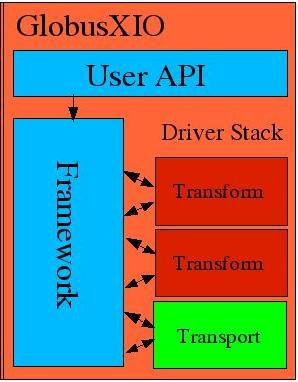
\includegraphics[width=3.4in]{figure1}}
\vspace*{-2.0ex}
\caption{Globus XIO Architecture}
\label{arch}
\end{figure}

Figure 1 show the architecture of Globus XIO.  The user interacts with 
the simple open/close/read/write API and posts data operations to it.
The Globus XIO framework then forwards the buffers along to the first
driver in the stack.  When then driver \emph{passes} the operation along
the framework forwards it to the next driver in the stack and so on
until the operation reaches the transport driver.  Once the transport 
driver has completed the operation it tells the framework it is 
\emph{finished}.  We refer to this as finishing an operation.  The 
framework then moves up the stack notifying each driver that the 
one below it is done with the task that was passed to it.  Drivers
are free to do some processing in between the time they are told
the lower driver finished and the time they finish the operation.

\section{Asynchronous C Programming}
Globus XIO is designed on an asynchronous model, therefore
the driver interface is designed on an asynchronous model as well.
The driver is signaled to perform a task.  It can complete this
task at anytime without regard for the thread of execution that
made the request.  When the driver completes the task it signals
the Globus XIO framework that it is finished.  That is the drivers 
asynchronous model in a nutshell.  

Explaining
proper asynchronous programming techniques is a task of its own.  We
do not intend to take on this task in this guide, however since 
understanding at least the basic ideas behind it are crucial to 
developing Globus XIO drivers we will briefly discuss it in this section.
Readers familiar with asynchronous programming should skip this section.

In C 101 we learn about the $main()$ function.  When an application 
begins a single thread starts executing instructions at the beginning
of the main function.  Execution continues, following branches, loops,
jumps to function etc.  As soon execution reaches the end of the $main()$
function it ends.  To the developer this model is very easy to follow.
Processing occurs sequential and the next line of code that will be executed
is very predicable.

The blocking models follows this way of thinking.  When a developer wishes
to read data from a socket they call the read() function.  Execution 
enters that function and does not return until it has read the data which
the user requested.  While in that function the users application 
blocks.  This is an easy and predictable means of performing IO, however
it is not the most efficient use of the CPU.  While waiting for data
to be read the CPU is largely idle and the application could very well
have work it to do that is independent of that read.  However, since
it is blocked in that function it can do nothing but wait.

The asynchronous IO model is much different.  Instead of blocking
for an operation to complete the developer \emph{registers} the IO event.
As part of the registration the developer passes in a function pointer.
When the event completes that function pointer is called.  So in 
asynchronous IO, many operations are posted and at any time an event
can take place that will cause their callback to fire.  The developer
must be prepared for the event to occur at any time after registration.
This can get very complicated in the face of a many simultaneous
operations.

Developers must be aware that many event callbacks could happen at the same
time.  Therefore they need to use mutexes to protect critical sections
of code.  In this model, as in any multithreaded programming model,
users must be careful of race conditions and deadlock situations.
The recommended approach in the asynchronous programming model is 
to use a finite state machine.  In this approach the developer 
identifies and enumerates all of the distinct states that a program 
can go through as well as all of the transitions from one of these
states to another.  When an event occurs the developer checks the current
state and the type of event against against this state machine to determine
what the next state to transition to will be.

\subsection{Example State Machine}
Here we take a look at a simple example.  Figure 2 shows a state machine
with the following states:
\begin{itemize}
\item START
\item OPENING
\item OPEN
\item READING
\item CLOSING
\item CLOSED
\end{itemize}

And the following transition events:
\begin{itemize}
\item open registered
\item open completes
\item read registered
\item read completes
\item close registered
\item close completes
\end{itemize}

\begin{figure}
\centerline{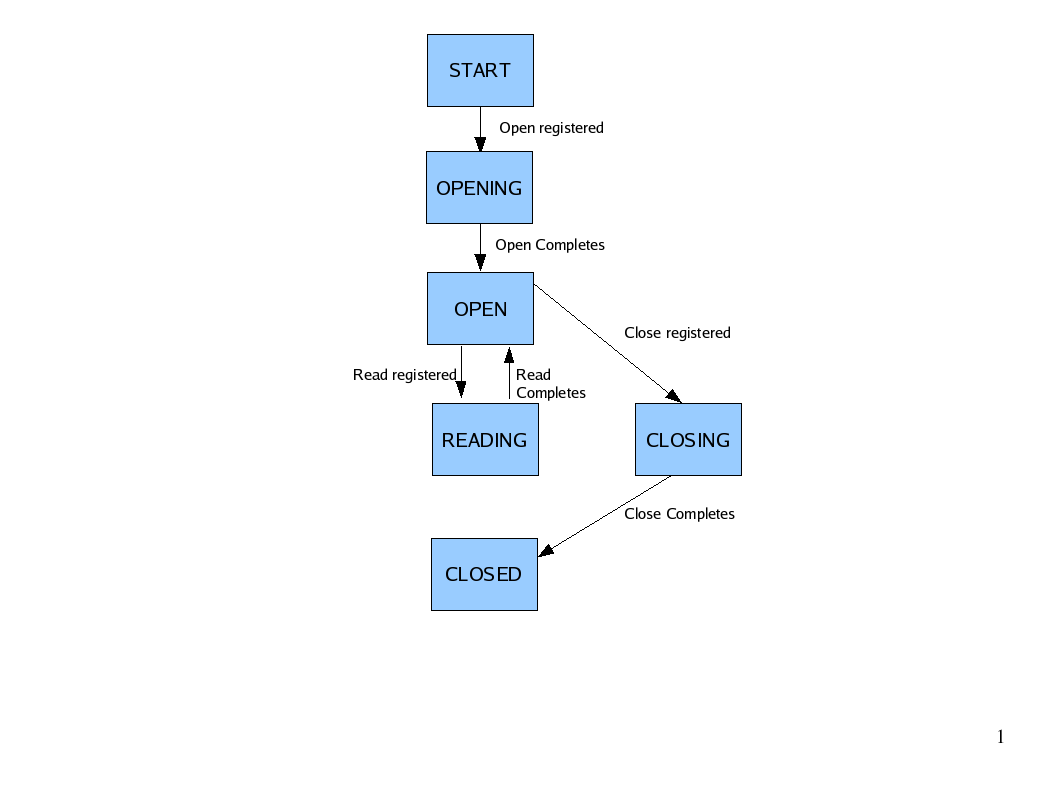
\includegraphics[width=3.4in]{figure2}}
\vspace*{-2.0ex}
\caption{Example State Machine}
\label{Example State Machine}
\end{figure}

As the diagram shows each the current state changes when an event takes
place.  When in any given state there is a set of possible transition events.
No event outside of that set is allowed to occur in that state.  The event
that does occur determines the next state.  It is recommended that an
asynchronous programmer starts by creating a state diagram like the one
shown in figure 2.  


For more information on asynchronous programming see:
\begin{itemize}
\item pthread manual
\item http://www.globus.org/toolkit/docs/3.2/developer/globus-async.html
\end{itemize}

\section{Driver Development Introduction}
In this section we explain how to make a Globus XIO driver.  A driver is 
a dynamically loadable C library with a well defined set of interface
functions.  
The interface functions are wrapped together in a in a data structure.
When a Globus XIO application chooses to load a driver it locates this
symbol in the shared library according to a naming convention.
The application gives Globus XIO a driver name, a driver with this name
is then searched for in the $LB\_LIBRARY\_PATH$.  If found the library is
loaded and the symbol containing the interface functions is acquired,
at which point Globus XIO has all it needs to use the driver.

All interface functions are expected to provide a well defined operation.
This can be viewed as a contract between Globus XIO and the driver.
For example, the \emph{read} function is expected to get new data
and give that data to Globus XIO.  It does not matter how the driver
does it.  The file driver will get the data from the file system, the
TCP driver will get the data from a socket.  The contract does not
care \emph{how} the data is acquired, it only cares that the driver
copy the data into the provided buffers.  In order to help the driver 
developer honor the interface function contracts
there is an assist API.  

Before we go into greater detail on the interface function, their contacts,
and all of the data structures that go along with it we first introduce
the reader to more general concepts in driver development and try to 
provide an understanding of the flow of a driver.
First we give a quick overview of how it works.  
The tricky bits and hardcore rules are left out for now.

\subsection{The Operation}
First we look at \emph{operations}.  The interface functions
represents a call from the framework to the driver requesting that some
specific operation be performed (for example, read/write/open/close).  
Since Globus XIO drivers are on an 
asynchronous model *(wrapblock), the driver may perform 
this operation on its own time.  The driver
is not expected to finish the operation withing scope of the interface
function call.  The driver is free to schedule the request for later, 
or perform the request in some low priority thread or in some other out
of band asynchronous function without stopping up the entire system.
Globus XIO signals the driver when it wants an operation
to be completed, and the driver signals Globus XIO when it has 
completed the operation.  Once receiving the start signal, the driver
can give the finished signal at anytime, and from any thread/callstack
that it likes.

Three things are needed to accomplish this signaling.  The first is the
interface function, which we have discussed.  This function is called
to signal the driver that an operation must be performed.  The second
thing required is an operation data type which encapsulates what operation
is in question.  This is just a type defined pointer to internal state
which is associated with the requested operation.  Finally we need 
an \emph{operation finished} function that the driver
may use to signal Globus XIO that it has completed it request.

Let us look at an example using a read operation.

\begin{verbatim}

globus_result_t
sample_read(
    void *                              driver_specific_handle,
    const globus_xio_iovec_t *          iovec,
    int                                 iovec_count,
    globus_xio_operation_t              op)
{
    /* driver specific code to appropriately fill in the iovec */

    globus_xio_driver_finished_read(op, GLOBUS_SUCCESS, nbytes);

    return GLOBUS_SUCCESS;
}

\end{verbatim}

In this oversimplified example $sample\_read$ will be called
by Globus XIO when an application requests a read via a call to
$globus\_xio\_read()$ and the like.  The first parameter to
$sample\_read$ is $driver\_specific\_handle$, this is a pointer
to driver defined memory.  We will look at this parameter in detail
later but for now we shall ignore it.  The next two parameters 
$iovec$ and $iovec\_count$ point to memory buffers into which
the driver is to read data.  Much information exists on iovec as it 
is a common BSD socket idiom.  And the final parameter is $op$.
$op$ is a Globus XIO data type that holds internal information about
the specific read operation called.  The driver developer must 
hang onto this operation data type until it has completed the request,
at which time it calls $globus\_xio\_driver\_finished\_read()$, passing
in $op$ and thereby signaling Globus XIO of its completion.

In the above example $globus\_xio\_driver\_finished\_read()$ \emph{is} called
with in the scope of the $sample\_read$ function.  This is only done
for example clarity, this in no way must be the case, and most often
it is not the
case.  The driver could copy the $globus\_xio\_operation\_t$ by using
the $=$ operator, return from the $sample\_read$ function and at any time
later call $globus\_xio\_driver\_finished\_read()$ passing in the copied
$op$.

The reader may also take note of the use of $GLOBUS\_SUCCESS$ in the example.
$GLOBUS\_SUCCESS$ is a value of a $globus\_result\_t$ which is used to
communicate success and failure.  Any value other that $GLOBUS\_SUCCESS$
indicates failure.  A $globus\_result\_t$ can take on many values to
communicate an error.  Details on Globus errors are documented 
elsewhere, for our purposes we only need to know that $GLOBUS\_SUCCESS$ 
is success and anything else is a failure.
The value  returned from the interface function indicates
if the driver is willing to \emph{attempt} to fulfill the request.  
$GLOBUS\_SUCCESS$ indicates that it is willing to try and an error
type indicates that it is not.  
If the interface function returns $GLOBUS\_SUCCESS$
it \emph{must} call $globus\_xio\_driver\_finished\_read()$ at a later time, 
passing in the given $op$.  If it returns
an error type it \emph{must not} call $globus\_xio\_driver\_finished\_read()$
with the $op$ and should further consider that $op$ invalid as soon as it
returns from the function.

Just because the driver said it was willing to try to fulfill the
request, it does not mean that it will be successful.  Since we are
dealing with an asynchronous model the driver may not know right away
if it can successfully fulfill the request.  If after returning 
$GLOBUS\_SUCCESS$ in the interface function some situation occurs 
which prevents the driver from servicing
the operation, the driver will call $globus\_xio\_driver\_finished\_read()$
passing in the given op and an error type in the place of $GLOBUS\_SUCCESS$
that indicates it failed in its attempt to complete the operation.

\subsection{Tying Operations Together}
In the previous section we introduced the $driver\_specific\_handle$ parameter
but delayed the discussion of it.  In this section it will play a 
prominent role.  IO operations are typically not self contained things.
In most cases they interrelate to each other.  As an example look at file
IO.  In order to read a file, you must first open it, and the current
read position depends on the previous read position.  Finally to clean up
you need to close the file.  All of these operations depend upon having some
shared state that each individual operation can check.  What this state
consists of will differ for each driver.  ...
some drivers user x, other uses y.  therefore it is the driver that must 
define this state.

we use the $driver\_specific\_handle$ for this.  at initialize time the
driver allocates a structure and returns a pointer to that structures
memory back to Globus XIO.  This pointer is then threaded through to all
operations via the $driver\_specific\_handle$.  To Globus XIO
$driver\_specific\_handle$ is just a void *, just a pointer to memory, so 
the driver must up-cast the void * back to its structure.  look at over-
simplified example:

\begin{verbatim}

typedef struct simple_file_handle_s
{
    FILE *                              fptr;
    ssize_t                             total_bytes;
} simple_file_handle_t;

globus_result_t
sample_open(
    const globus_xio_contact_t *        contact_info,
    void *                              driver_link,
    void *                              driver_attr,
    globus_xio_operation_t              op)
{
    char *                              filename;
    simple_file_handle_t *              handle;

    handle = (simple_file_handle_t *) malloc(sizeof(simple_file_handle_t));

    filename = contact_info->resource;
    handle->fptr = fopen(filename, "r");
    handle->total_bytes = 0;
                   
    globus_xio_driver_finished_open(handle, op, GLOBUS_SUCCESS);

    return GLOBUS_SUCCESS;
}

globus_result_t
sample_write(
    void *                              driver_specific_handle,
    const globus_xio_iovec_t *          iovec,
    int                                 iovec_count,
    globus_xio_operation_t              op)
{
    globus_size_t                       nbytes = 0;
    int                                 i;
    simple_file_handle_t *              handle;

    handle = (simple_file_handle_t *) driver_specific_handle;

    /* walk through iovec and write all the bytes */
    for(i = 0; i < iovec_count; i++)
    {
        nbytes += fwrite(iovec[i].iov_base, 1, iovec[i].iov_len, handle->fptr);
    }
    handle->total_bytes += nbytes; /* keep the overall total */

    globus_xio_driver_finished_write(op, GLOBUS_SUCCESS, nbytes);

    return GLOBUS_SUCCESS;
}

globus_result_t
sample_close(
    void *                              driver_specific_handle,
    void *                              attr,
    globus_xio_operation_t              op)
{
    simple_file_handle_t *              handle;

    handle = (simple_file_handle_t *) driver_specific_handle;

    fclose(handle->fptr);
    free(handle);

    globus_xio_driver_finished_close(op, GLOBUS_SUCCESS);

    return GLOBUS_SUCCESS;
}


\end{verbatim}

In this example we show how state is maintained across the open, close,
and write interface functions.  The reader should note that this is
a greatly over simplified example for the purpose of explanation.  It is
not intended to actually work as a Globus XIO driver, but rather is intended
for didactic purposes.  In this example all processing is done in line in a
blocking fashion.  This is $not$ typical for Globus XIO driver, but makes for
a much more compact example.

In the example the data structure $simple\_file\_handle\_t$ is allocated
and initialized in the open function.  Since this is a very basic file
driver example we open a file and put the $FILE *$ in the 
$simple\_file\_handle\_t$.  We get the file name that the user wishes to
open from the $contact\_info$ structure.  More details on that can be found
in the user API. XXX no it can't... this is a driver structure only * XXX
To show that multiple data members can be useful in a
$driver\_specific\_handle$
we keep a running total of the number of bytes written in the handle as well.
Once open we \emph{finish} the open operation with a call to
$globus\_xio\_driver\_finished\_open()$.  The first parameter to this function
is the pointer to the $simple\_file\_handle\_t$.  Globus XIO will associate
that pointer with all operations called upon this handle and pass this 
pointer into all other operations associated with this handle.

Notice how the $driver\_specific\_handle$ is passed into $simple\_write()$
where the $void *$ is cast back into a $simple\_file\_handle\_t *$.  The
driver now has access to the needed $FILE *$ and it uses it to write the 
data in the iovec array to the file.  The driver keeps track of all
the bytes it has written and passes that number into 
$globus\_xio\_driver\_finished\_write$ along with the operation to 
tell Globus XIO exactly how much of the write that it has completed.  
In this example we ignore all possible errors for the purpose of simplicity.
The driver is allowed to return a short value for nbytes if it wishes.

The $driver\_specific\_handle$ is also passed into the close function.
The close function is the final operation that will be requested on this 
handle so it is where all of the associated memory is cleaned up.  We
again cast the $void *$ to a $simple\_file\_handle\_t *$.  We then call 
$fclose()$ to close the file and free memory pointed to by the handle.
Finally $globus\_xio\_driver\_finished\_close$ is called and the driver has 
completed its use of this handle.

\subsection{Passing}
The previous section gives an overview of the general flow of control
in a driver.  Specifically it shows the interactions of a \emph{transport}
driver.  We know it is a \emph{transport} by two things described above.
The first is that it is doing the actual work of transporting the data
outside of the process space (in this case across the kernel boundary) 
with the call to $fwrite()$.  The second way is that it doesn't rely
on any other driver for help.  In this section we show how drivers 
can be written such that they do rely on other drivers to help service
their requests.

A \emph{transform} driver can delegate the responsibility of completing
part, or all of an operation to the next driver down the stack.  We call
this \emph{passing} an operation.  To illustrate this process we will
look at another simple example.  
In this example we will create a $simple\_zip$ transform driver.  This
driver will compress data buffers and then pass the new buffers down the 
stack.  The next driver in the stack could be anything at all, the 
$simple\_zip$ driver doesn't know or care what is next, it only knows
that it can ask the next driver to open/close/read/write (and a few other 
operations discussed later) on its behalf.

For clarity the reader can consider the stack to be a the $simple\_zip$
driver on top of the $simple\_file$ driver.  This would result in a stack
that writes compressed data to a disk.  However, the example should make it
clear that the $simple\_zip$ driver could be mixed and matched with any 
valid driver set.  In the example we will use an imaginary function that 
when given a buffer and a length it will return a new buffer and length
that contains the compressed data of the first.

\begin{verbatim}

typedef struct zipped_data_s
{
    globus_xio_iovec_t *                iov;
    int                                 iovc;
} zipped_data_t;

globus_result_t
zip_open(
    const globus_xio_contact_t *        contact_info,
    void *                              driver_link,
    void *                              driver_attr,
    globus_xio_operation_t              op)
{
    globus_result_t                     result;

    result = globus_xio_driver_pass_open(op, contact_info, NULL, NULL);

    return result;
}

void
zip_write_cb(
    globus_xio_operation_t              op,
    globus_result_t                     result,
    globus_size_t                       nbytes,
    void *                              user_arg)
{
    int                                 i;
    zipped_data_t *                     zipped_data;

    /* clean up */
    zipped_data = (zipped_data_t *) user_arg;
    for(i = 0; i < zipped_data->iovc; i++)
    {
        free(zipped_data->iov[i].iov_base);
    }
    free(zipped_data->iov);
    free(zipped_data);

    globus_xio_driver_finished_write(op, result, nbytes);
}

globus_result_t
zip_write(
    void *                              driver_specific_handle,
    const globus_xio_iovec_t *          iovec,
    int                                 iovec_count,
    globus_xio_operation_t              op)
{
    int                                 i;
    globus_size_t                       nbytes = 0;
    zipped_data_t *                     zipped_data;

    zipped_data = (zipped_data_t *) malloc(sizeof(zipped_data_t));
    zipped_data->iovc = iovec_count;
    zipped_data->iov = calloc(iovc, sizeof(zipped_data_t);

    /* walk through iovec and write all the bytes */
    for(i = 0; i < iovec_count; i++)
    {
        /* a fake function the compresses the first buffer into the 2nd */
        simple_zip(
            iovec[i].iov_base, iovec[i].iov_len,
            &zipped_data->iov[i].iov_base, &zipped_data->iov[i].iov_len);
        nbytes += zipped_data->iov[i].iov_len;
    }

    result = globus_xio_driver_pass_write(op, zipped_data->iov,
        zipped_data->iovc, nbytes, zip_write_cb, zipped_data);

    return result;
}

globus_result_t
zip_close(
    void *                              driver_specific_handle,
    void *                              attr,
    globus_xio_operation_t              op)
{
    globus_result_t                     result;

    result = globus_xio_driver_pass_close(op, NULL, NULL);

    return result;
}

\end{verbatim}

The first thing to notice in this example is the use of the \emph{pass}
functions.  For starters lets look at the \emph{open} and \emph{close}
interface functions.  Since the imaginary compression library used in this
example doesn't require any state we do not have to thread 
$driver\_specific\_handle$ through all of the interface functions and thus
$zip\_open$ and $zip\_close$ do very little.  In fact, the only thing they
do is \emph{pass} the operation off to the next driver.  If the zip driver
wanted to know when the open completed it could pass a function
pointer in as the second argument to $globus\_xio\_driver\_pass\_open()$ and
that function would be called upon completion.  However since it does
not need to know the example simply passes NULL in for this parameter.
As soon as the operation is passed down the stack the $zip$ driver is 
done with it and relies on the other drivers in the stack to complete
the operation.

The write interface function is slightly more complicated.  The job of
this function is simply to compress the data and then send it down the stack.
However, since the driver cannot alter the users buffers, it must create
new buffers for the compressed data to reside.  This is done by creating
the $zipped\_data\_t$ structure.  In it is an iovec with the same number 
of entries as the users iovec.  For each of the entries $simple\_zip$ is
called to create the zipped buffer.  Once all of the zipped buffers are
created they can be passed down the stack with 
$globus\_xio\_driver\_pass\_write()$.  Unlike with open and close, here we
must know when the write has completed so that we can free this
memory.  We cannot free the memory before the write has completed or
we will corrupt the system memory, and if we never free it we will leak
memory.  Therefore we have to pass a pointer to the function 
$zip\_write\_cb()$ (\emph{cb} stands for \emph{callback}).  Once the
write operation has been completed by the remainder of the driver stack
that function will be called and we can free memory.  $zip\_write()$ frees
the memory and then calls $globus\_xio\_driver\_finished\_write$ to notify
Globus XIO that it has completed the operation it was asked to do.

\subsection{Servers}
There are two sides to most connections: the active side and the passive side.
The active side is the well known one that decides when the connection
will take place.  It initiates a open with an endpoint (listening port 
or file name) and immediately the connection begins to be established.
A passive open is a little less known, or at least less considered.  The
passive side of a connection is one in the listening state.  It begins
the opening process by creating a listener and then waiting for some
period of time a remote active connection to contact it.  It does not
complete the open process until it is contacted.  The passive contact
point is sometimes referred to as a $server socket$ or just a $server$.

Often the server will be used for creating many connection.  It does a
passive open and publishes its contact point.  $Clients$ 
can then perform an active open to that contact point.  Once one connection
is established the server can continue to listen on the same contact point
for additional connection requests.  This is a common approach to
passive opens and one that is taken in Globus XIO.

Servers in Globus XIO use the same asynchronous model and the same driver
interface model.  To create a driver that can operate as a server the
developer must implement three interface functions in addition to the 
ones described above.  The functions are:

\begin{verbatim}

typedef globus_result_t
(*globus_xio_driver_server_init_t)(
    void *                              driver_attr,
    const globus_xio_contact_t *        contact_info,
    globus_xio_operation_t              op);


typedef globus_result_t
(*globus_xio_driver_server_destroy_t)(
    void *                              driver_server);

typedef globus_result_t
(*globus_xio_driver_server_accept_t)(
    void *                              driver_server,
    globus_xio_operation_t              op);

\end{verbatim}

The first two interface function will be called when a user of the Globus
XIO API creates and destroys a server.  The interface calls give the driver
developer an opportunity to allocate resources associate with that server.
When the driver receives a call to its $server_init()$ funciton, it 
creates memory, and listeners and whatever else it needs to perform
its driver specific server tasks, and the makes a call to:

\begin{verbatim}

globus_result_t
globus_xio_driver_pass_server_init(
    globus_xio_operation_t              op,
    const globus_xio_contact_t *        contact_info,
    void *                              driver_server);

\end{verbatim}

This tells Globus XIO that the driver has completed setting up the server.
The driver will be listening at the contact point described by the 
second parameter to the function, and all future references to this 
server will come with the pointer to user memory in the third parameter,
$driver_server$.

When $globus_xio_driver_server_destroy_t()$ is called the driver must clean
up all resources associated with the user memory pointer.  It is a 
synchronous call so the driver does not need to call any further function
to signal completion.  It is assumed that when the driver returns from the
function it has completed cleaning up resources.

The $globus_xio_driver_server_accept_t$ interface function is where the 
interesting work takes place.  This is called when a server has received
a connection request from a client.  Here the driver prepares a new 
connection handle as it would when an active open occurs.  Once complete
it calls:

\begin{verbatim}

globus_result_t
globus_xio_driver_pass_accept(
    globus_xio_operation_t              op,
    globus_xio_driver_callback_t        in_cb,
    void *                              in_user_arg);

\end{verbatim}

This signals to Globus XIO that the driver is passing the accept request
down the stack.  When the remaining drivers in the stack have completed
their portion of the accept the callback given in the second parameter
will be called.  Once that callback is called the driver can complete
its accept with a call to:

\begin{verbatim}

void
globus_xio_driver_finished_accept(
    globus_xio_operation_t              op,
    void *                              driver_link,
    globus_result_t                     result);

\end{verbatim}

If the the driver is a transform driver it does not call 
$globus_xio_driver_pass_accept()$.  It simply does everything required 
it self and then calls $globus_xio_driver_finished_accept()$ when complete.

\subsection{Driver Specific Optimizations}
TODO

\section{Driver Development Manual}
TODO

\subsection{Guidelines}
%the real rules
%finished outside of locking
%when callback can occur
%serialized calls
%life time of operation

%\subsection{cancels}

%\subsection{Data Descriptors}
%very brief explanation of concept.  perhaps show how mode e uses them

%\subsection{Driver Operations}
%again brief introduction
%how used in out of band stuff
%advanced tequs

%\subsection{Using user api to implement driver}

\section{Wrapblock}
Todo

\section{Summary}
TODO

\section*{Acknowledgements}
TODO

\end{document}
